\chapter{Prototype "Julep Search"}
\label{cha:prototypejulepsearch}

In this final chapter of this thesis the reader will be introduced to the prototype that was developed during the research time of this paper. The understanding of all topics that were presented in this thesis should be greatly improved by going over an actual practical example of a real world ReactJS web application. Many best practice and application architecture suggestions are based on the practical experience that was collected during the development of the prototype.

\section{Introduction to the project}

First there will be an introduction to what Julep Search actually is about and what the tool is trying to achieve. This prototype partly was developed while working in an internship at a small web agency in Vienna which is called \enquote{Agentur Mint}\footnote{https://www.agentur-mint.com/}. One branch of this company called \enquote{Mint Square}\footnote{https://www.mint-square.com/} is supporting companies with programmatic advertising know-how and and consultancy. The prototype which is presented is a tool which was built for this branch of the Mint agency to alleviate the tedious process of searching large databases for client specific programmatic advertisement data.

\subsection{Motivation}

Mint Square actually has a database for many different advertising platforms and at one point in time there was the need for a tool that could sort and visualize large amounts of raw advertisement information data. That data can be used to optimize the placement of advertisements and help companies to specifically put advertisements on spots that are most relevant to be noticed and realized by the users. This process is called \enquote{programmatic advertisement}.

The motivation is to easily process programmatic advertisement data  that can then further processed by the collaborators of the Mint-Square team. The most important requirement is to make all data searchable by embedding data into an interface that is easily operable.

\subsection{Usecase}

Once a company wants to start using programmatic advertising for their web appearance it is necessary to get some information what kind of advertisement would work best in what kind of situation. The target audience has to be evaluated and also what advertisements would work best for that audience. This tool queries a large database for all kinds of key information. For example there are queries for keywords, categories, or inventories. The results then show the corresponding advertisement providers, their request counter and additional information that can be used by the employees of Mint Square to evaluate whether the advertisement provider is valid or not.

\subsection{Used technologies} \label{ssec:usedtechnologies}

The application itself is a staticly served single page application built with ReactJS. It is hosted on an Amazon S3 bucket, which is a simple static file hosting server that is extremely cheap to operate. As it was explained before in this paper, bundling a web application by technologies like Webpack makes it easy to host the application on any platform as only static files have to be served to the client.

The database that contains all relevant advertisement data is an Amazon Elastic Search container\footnote{https://www.elastic.co/}. Elastic search is a database that makes querying data with special context very easy. It has a built in matching percentage algorithm that lets the programmer query the most relevant data and also sort the data after its relevancy.

Julep Search does not need a back end server other than its database. For this project a serverless\footnote{https://serverless.com/} approach was chosen. Serverless is a technology that makes heavy use of Amazon's lambda functions completely omitting the necessity to operate a server for any API calls. Lambda functions won't be explained in this paper as it would go beyond the scope of this paper. Information about Amazon's lambda functions can be read on Amazons official documentation\footnote{http://docs.aws.amazon.com/lambda/latest/dg/welcome.html}.

\section{The prototype}

When designing the prototype the most important goal was to implement a ReactJS web application that conforms to all best practices at the time (summer 2016). The emphasis was to have a code base that is easily readable and maintainable once the project is not actively maintained by the initial developer anymore. This section will give a quick overview over the most important aspects of the prototype and explain all thought and architectural decisions that were made.

\subsection{Architecture} \label{ssec:protarchitecture}

\begin{figure}
  \centering
  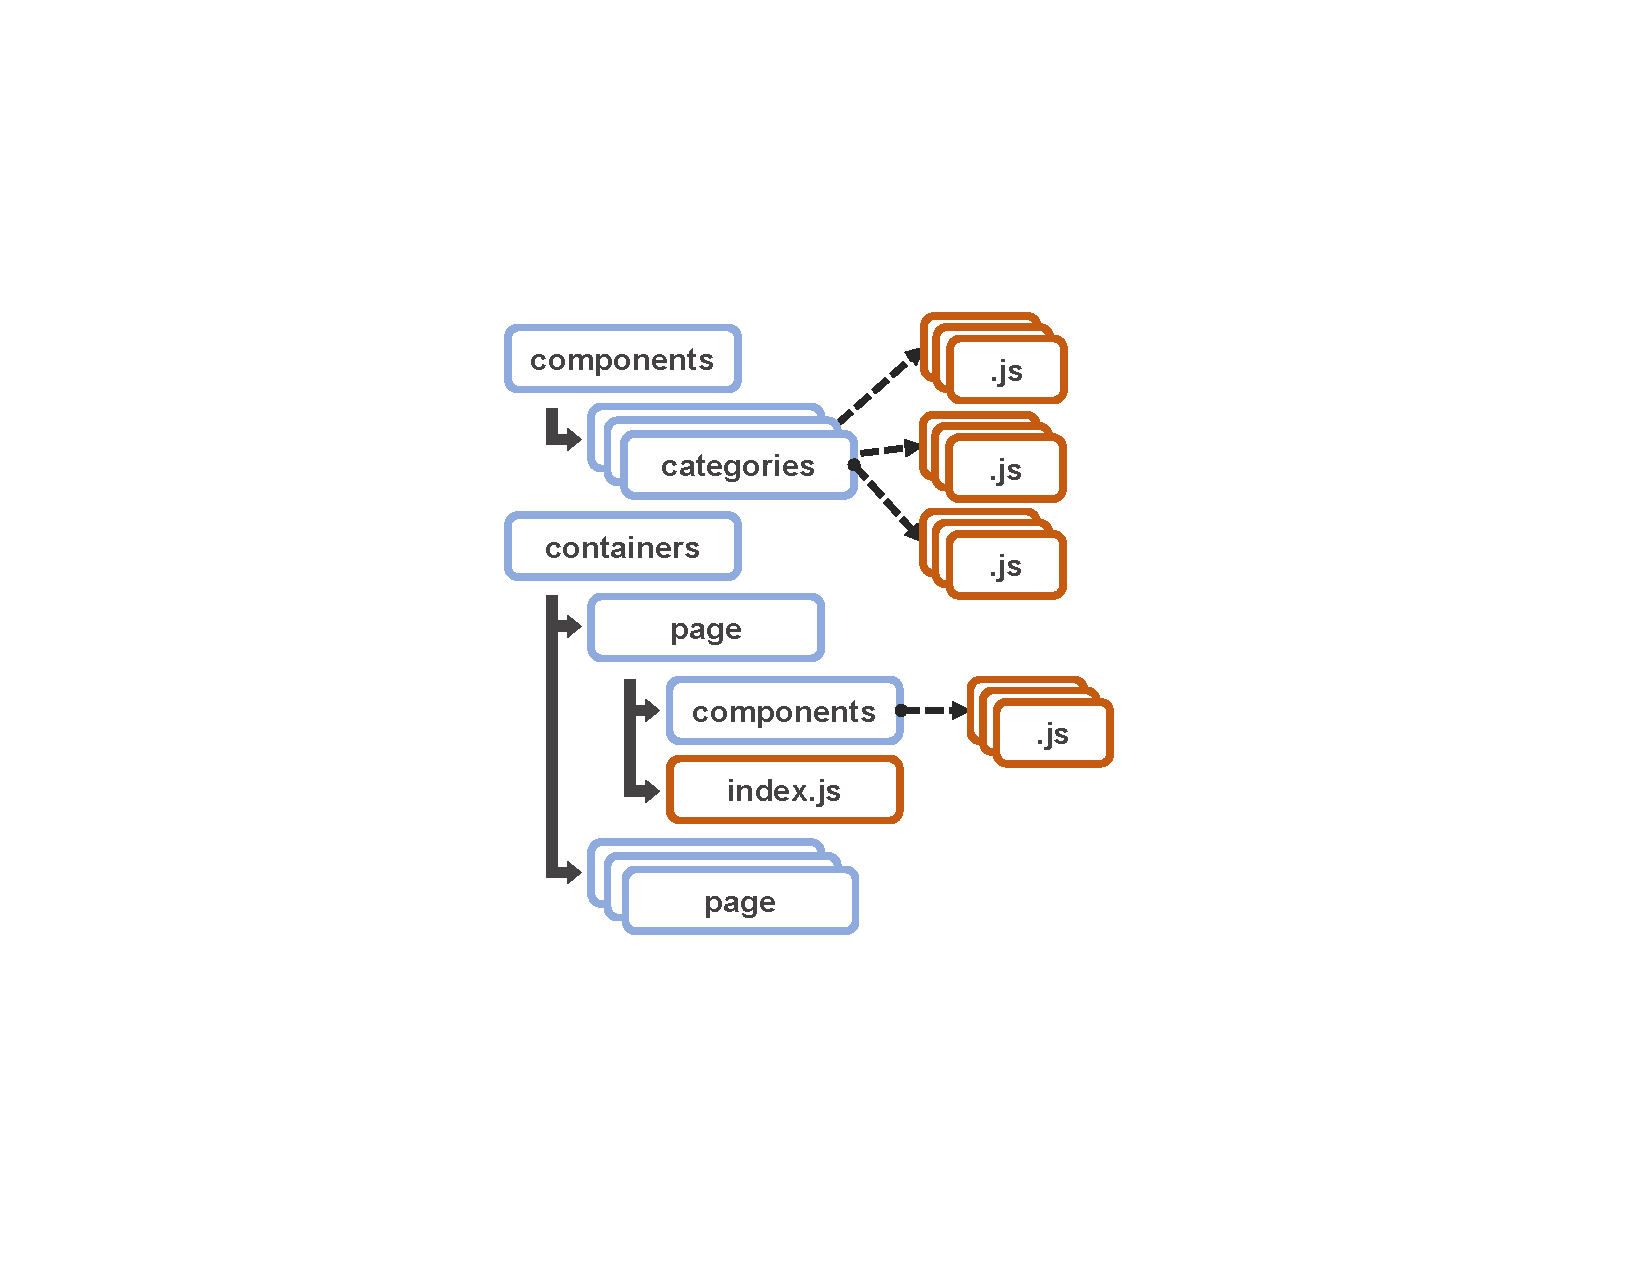
\includegraphics[scale=0.55, trim= 5cm 5cm 5cm 5cm, clip]{010architectureold}
  \caption{Basic application architecture}
  \label{fig:architectureold}
\end{figure}

The prototype was implemented keeping all best practices in mind that were explained in the Section \ref{sec:application-architecture}. In real world applications it is very complicated to entirely realize all best practices. The architecture of the prototype is also a little bit out of date as it was developed in summer 2016 and newer best practices and newer community standards have arisen until the time of this writing (May 2017).

The basic architecture of the application splits all parts into containers and components. Like mentioned before, the used application architecture is slightly out of date but it also more or less divides components into smart and dumb components. The Figure \ref{fig:architectureold} shows the prototype's current architecture. Every screen of the application has its own container section. The fact that all pages are divided into their own containers makes it easy for Webpack to codesplit the application bundle to prevent the user from having to download the complete application code if only the login screen is shown.

The biggest caveat of the current architecture is that every container still has its own specific components that are only used by that very container as the Figure \ref{fig:architectureold} tries to visualize. Application logic is scattered across multiple components which makes the whole application more difficult to understand. Oftentimes it is unclear what component of the container is connected to the store and what component handles which part of the container's logic. The solution to that problem is explained later in the Section \ref{ssec:donebetter}.

The components section of the application contains all UI elements that can be used to render simple components like a button or a text input component. As mentioned in the Chapter \ref{sec:application-architecture} the whole application should be expendable by only using existing UI components from the component library.

\subsection{Component}

As mentioned before it is very important to split the application into logical components that can be reused. A good example for a simple component would be the button component. The component wraps additional functionality around the native button DOM element that can be used throughout the whole application more comfortable and do avoid code duplication. The following example shows the basic button component of the prototype:\newline

\begin{JsCode}
/* ========================= LOAD modules =========================== */

import React, { PropTypes } from 'react'
import classNames from 'classnames'

/* ================================================================= */

const Button = (props) => {

  const className = classNames('button', props.className, {
    'button-primary': props.primary,
    'button-secondary': props.secondary,
    'button-disabled': props.disabled,
    'button-success': props.success,
    'button-failure': props.failure,
  })

  return (
    <button
      className={className}
      onClick={props.onClick}
    >
      {props.children}
    </button>
  )
}

Button.propTypes = {
  onClick: PropTypes.func.isRequired,
  className: PropTypes.string,
  primary: PropTypes.bool,
  secondary: PropTypes.bool,
  disabled: PropTypes.bool,
  success: PropTypes.bool,
  failure: PropTypes.bool,
}

export default Button
\end{JsCode}

In the prototype buttons can have multiple appearance variances. For instance, a button can be disabled or have a primary or secondary appearance. This can easily be controlled via \enquote{props} in ReactJS. In the following example the button can have many different properties that control how the button looks like. The \texttt{Button.propTypes} object shows, what properties can be set in order to change the appearance of the component. One example would be the \texttt{primary} property that transforms the button into a primary look. The \texttt{Button.propTypes} object also shows, that none of the properties is required so the button has a standard fall-back appearance if no property is set.

The property \texttt{onClick} has to be a callback function that gets executed when the button is pressed. The static \texttt{propTypes} object of the Button component has an \texttt{onClick} property that is set to \texttt{PropTypes.func.isRequired} which requires the property to be a function that must not be undefined when the component is used. Every time the button component gets clicked, React will handle the event and execute the passed callback function which has to be implemented by the user of the Button component in order to trigger some application logic.

Last but not least there is an implicit property that can be set. If a React component has children, they automatically get attached to the properties of the parent element. The children can be accessed in the parent component via \texttt{props.children}. This enables the component to process its children before embedding or rendering them. React provides a top-level API which can modify or rearrange children as it can be read in React's documentation \cite[React]{FacebookInc.2013}

\subsection{Container}

The following example shows how a standard stateful component looks like in ReactJS:\newline

\begin{JsCode}
/* ========================= LOAD modules =========================== */

import React, { Component } from 'react'
import { bindActionCreators } from 'redux'
import { connect } from 'react-redux'
import { 
  initialLoad, 
  updateFilterCriteria, 
  updateData, 
  exportData 
} from 'store/actions/data'

/* ======================= LOAD components ========================== */

import FlexContainer from 'components/common/flexContainer'
import DataTableView from './dataTableView'
import FilterCriteria from './filterCriteria'

/* ================================================================== */

const mapStateToProps = (state) => {
  return ({
    data: state.data,
    user: state.user,
  })
}

const mapDispatchToProps = (dispatch) => {
  return (
    bindActionCreators(
      {
        initialLoad,
        updateFilterCriteria,
        updateData,
        exportData,
      },
      dispatch,
    )
  )
}

class SearchDomainsPage extends Component {

  componentDidMount() {
    this.props.initialLoad()
  }

  componentWillReceiveProps(nextProps) {

    const filter = this.props.data.get('filter')
    const nextFilter = nextProps.data.get('filter')

    if (!filter.equals(nextProps.data.get('filter'))) {
      this.props.updateData(nextFilter)
    }
  }

  render() {

    // the properties are "destructured" from the this object
    // destructuring is an ES6 feature
    // the data, updateFilterCriteria and the exportData variables are extracted
    const { props: { data, updateFilterCriteria, exportData } } = this

    return (
      <div className="domain-search-page">
        <FlexContainer>
          <FilterCriteria
            updateFilterCriteria={updateFilterCriteria}
            data={data}
          />
          <DataTableView
            exportData={exportData}
            data={data}
          />
        </FlexContainer>
      </div>
    )
  }
}

export default connect(
  mapStateToProps,
  mapDispatchToProps,
)(SearchDomainsPage)
\end{JsCode}

Note how the component is connected to the Redux store of the application at the end where the component gets exported. In this advanced example the full potential of Redux is used as also the store's actions are bound to the component's properties. This feature was not described in this thesis as it would have gone beyond the scope. To learn about \texttt{react-redux}'s full potential the documentation can be read \footnote{https://github.com/reactjs/react-redux}.

The \texttt{componentWillReceiveProps} method is implemented which can react to the passed props of this component. If there was an update in the advertisement filter that queries the elastic search cluster the component will update itself via the provided callback function \texttt{updateData()} that has to be passed as prop to the component.

Because this component is a stateful component it provides the data from the store to all of its child components that are mostly dumb or stateless components in this case.

% \subsection{Important code examples}

% show some interesting code examples
% should component update
% smart dumb components
% handling state
% redux examples

\subsection{User interface explanation and demo}

The basic screen in Figure (\ref{fig:julep002}) shows the basic user interface. Some search criteria has already been applied and a list of domains and its corresponding relevant data is displayed. The list is sorted by the number of advertisement requests each domain gets. The panel \enquote{search criteria} can be used to refine the search parameters to enable more granular searches of the database. All results can also be exported as CSV files by clicking the \enquote{EXPORT} button in the top right corner of the results panel.\newline

\begin{figure}[H]
  \centering
  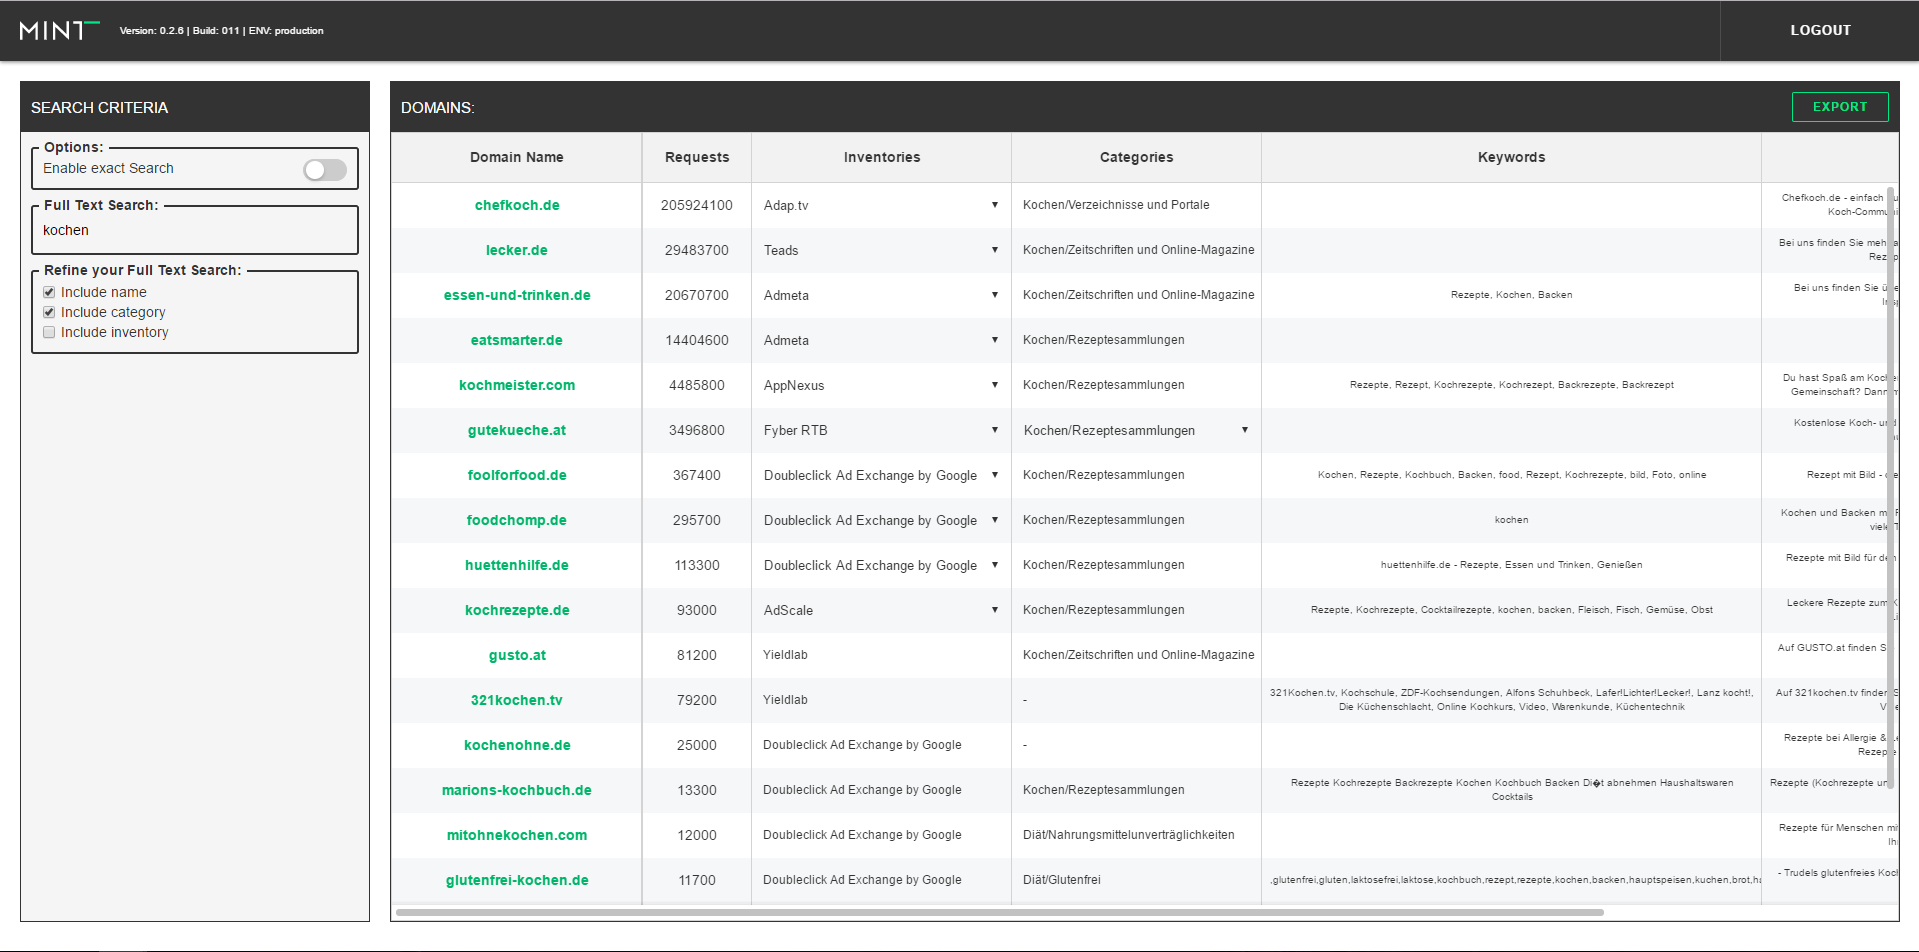
\includegraphics[width=15cm]{julep002}
  \caption{Applied search criteria in normal search}
  \label{fig:julep002}
\end{figure}

The following screen in Figure \ref{fig:julep003} shows a mockup of how the exact search could look like. As this is only a prototype the functionality was not fully implemented yet as there was no immediate demand for the feature.\newline

\begin{figure}[H]
  \centering
  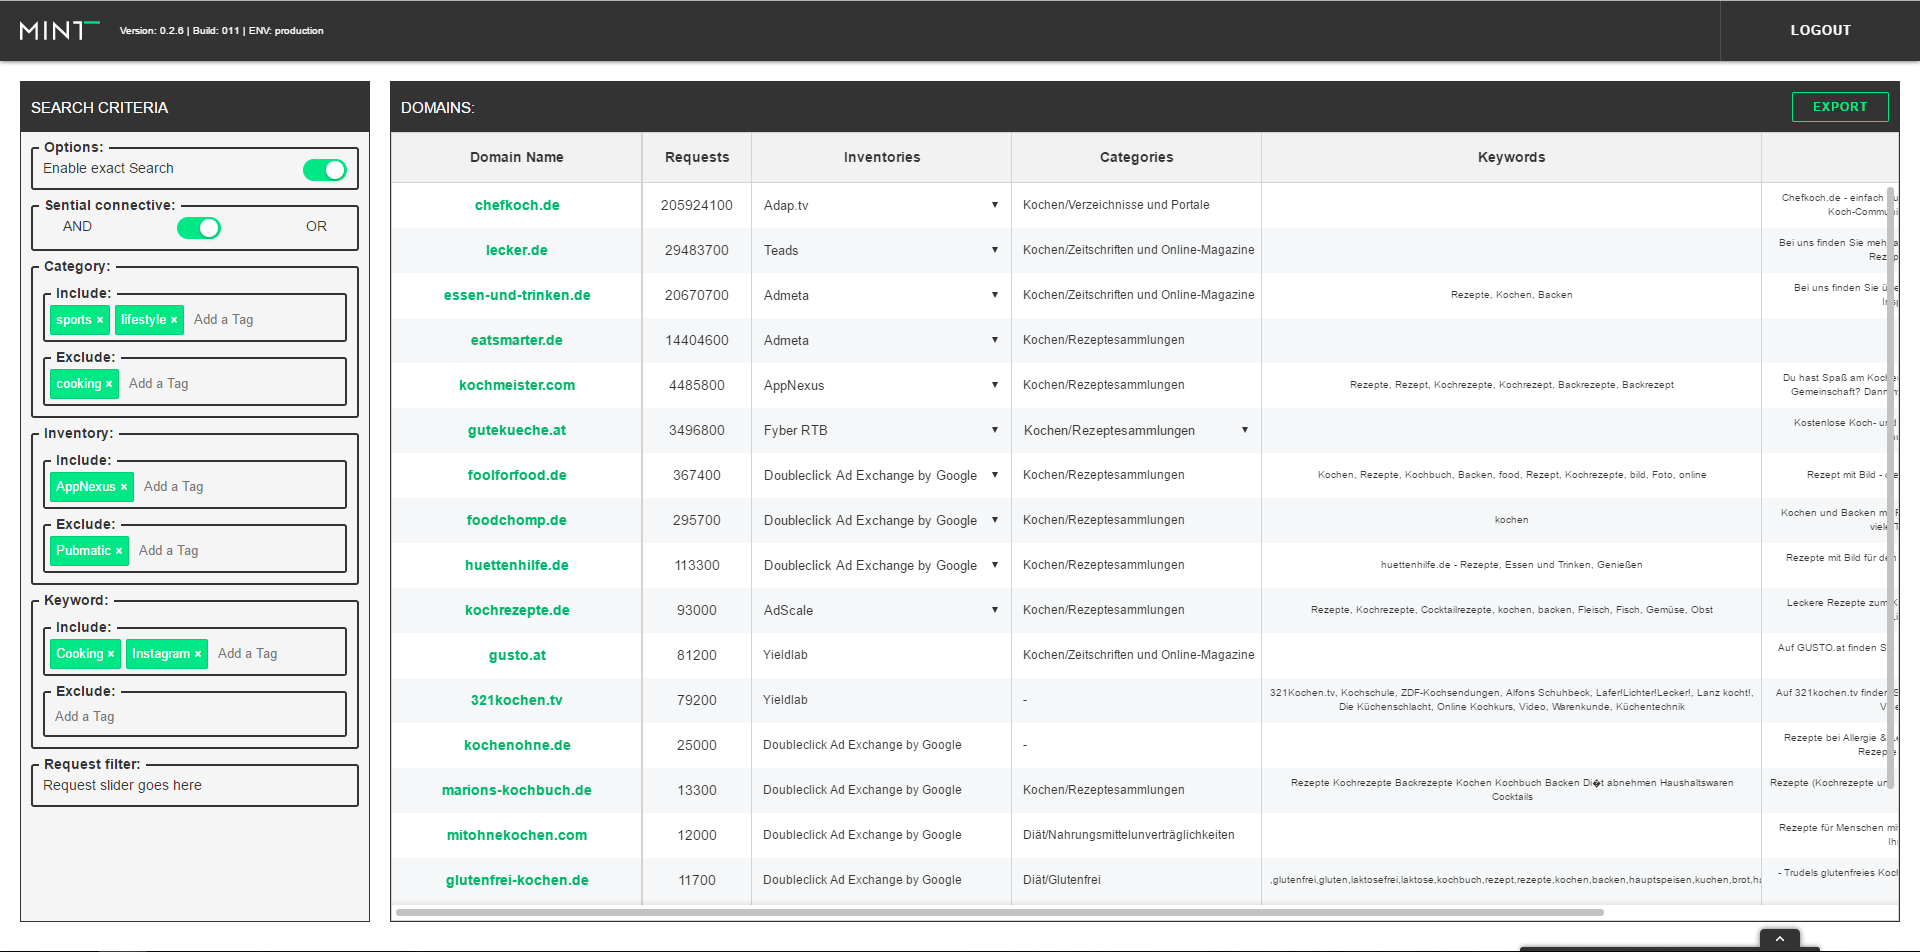
\includegraphics[width=15cm]{julep003}
  \caption{How the exact search could look like, only UI is implemented}
  \label{fig:julep003}
\end{figure}

To get a better overview over the search criteria panel, the following Figure \ref{fig:julep004} provides a better overview of the two different panels. On the left there is the basic search and on the right there is the basic implementation of the exact search panel, that does not have any logic attached to it yet.\newline

\begin{figure}[H]
  \centering
  \subfigure[normal search]{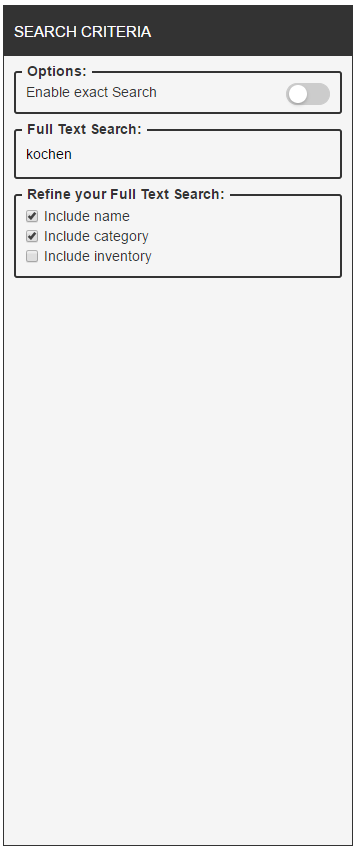
\includegraphics[height=14cm]{julep005} \label{fig:Raumeigner}} 
  \hspace{3cm}
  \subfigure[exact search]{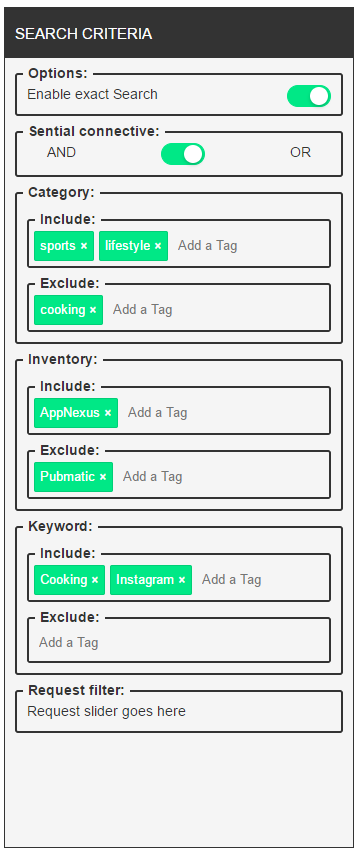
\includegraphics[height=14cm]{julep004} \label{fig:Raumverfügbar}} 
  \caption{Normal and exact search view} 
  \label{fig:julep004}
\end{figure} 

\subsection{What could have been done better} \label{ssec:donebetter}

\begin{figure}
  \centering
  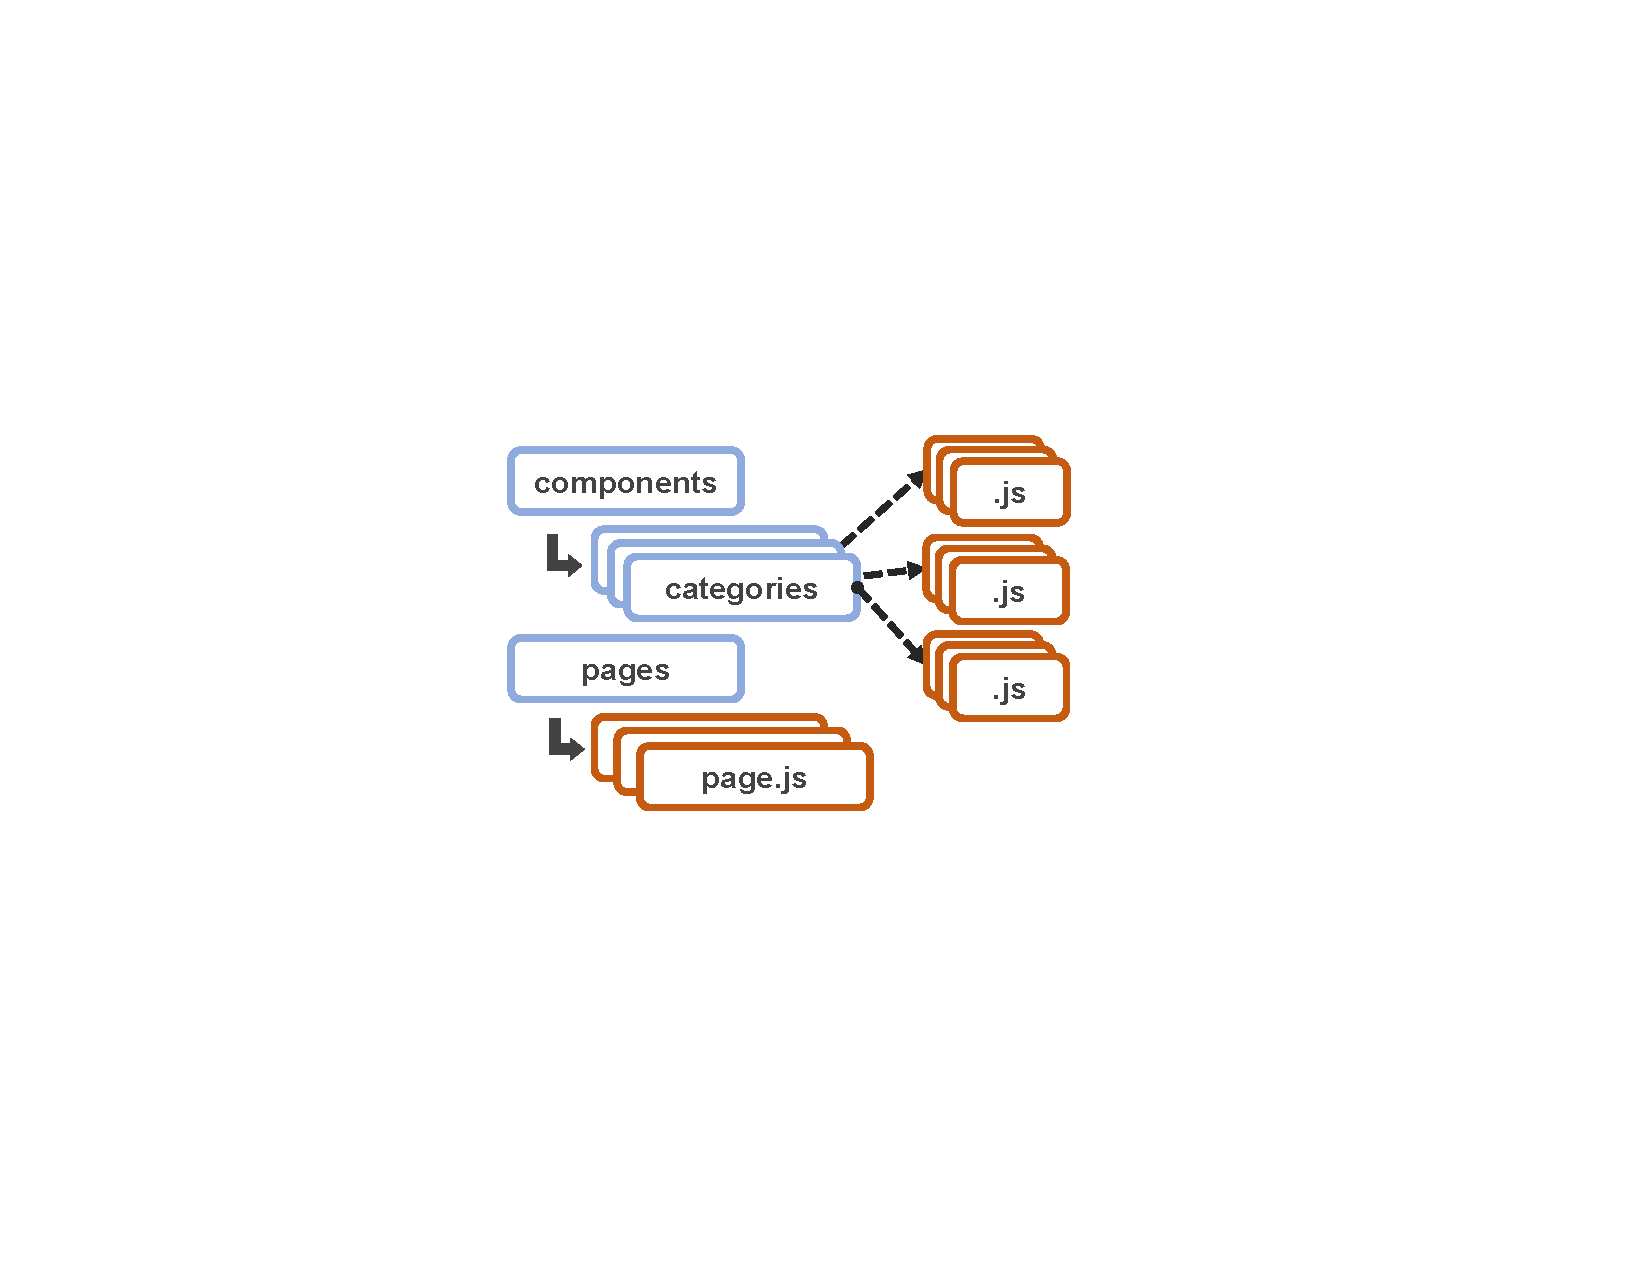
\includegraphics[scale=0.6, trim=5cm 7cm 5cm 7cm, clip]{011architecturenew}
  \caption{Better application architecture}
  \label{fig:architecturenew}
\end{figure}

In 2017 a new community standard arose that describes how to structure ReactJS applications as the Figure \ref{fig:architecturenew} shows. The whole application is divided into pages that can only use components from the component library. This should encourage developers even more to handle state and state-related logic only in one component (being the page component in this case) and pass all necessary logic down to the child components. This ensures that application-relevant logic is only handled in page components making the application much more easy to understand and to maintain.

As stated in the Section \ref{ssec:protarchitecture}, the prototype uses the slightly outdated application architecture that can be seen in the Figure \ref{fig:architectureold} that makes it noticeably more difficult to quickly understand the whole application logic. As the project is not maintained anymore the application was not refactored. The finding that the newer version of the application architecture can alleviate maintenance problems has to be kept in mind during the development of future projects.

% state what could have been done better, where errors have been made

% \subsection{There is still room for improvements}

% how could this application be improved? what is the future of this application?
% community -> page and components
% only connect page components to the store




